% !TEX recipe = pdflatex → bibtex → pdflatex × 2
%%
%% Agentic AI Paper — Artificial Intelligence (Elsevier) Submission
%% Paper #1 in the AI Systems Landscape 2026 series
%%
%% Artificial Intelligence (AIJ) formatting:
%%   - Uses Elsevier elsarticle document class
%%   - Author-year citations (natbib, authoryear style)
%%   - No strict word limit
%%   - Standard numbered sections
%%   - Review (double-spaced) layout for submission
%%
%% Preprint: engrXiv DOI 10.31224/6738 (March 2026)
%%

%% ================================================================
%% DOCUMENT CLASS — Elsevier Article
%% ================================================================
%% Options:
%%   review      = Double-spaced review format (required for submission)
%%   authoryear  = Author-year citation style
%%
\documentclass[review,authoryear]{elsarticle}

%% ================================================================
%% PACKAGES
%% ================================================================
\usepackage{graphicx}
\usepackage{multirow}
\usepackage{amsmath,amssymb,amsthm}
\usepackage{booktabs}
\usepackage{tikz}
\usetikzlibrary{shapes.geometric, arrows.meta, positioning, calc, fit, backgrounds, decorations.pathreplacing}
\usepackage{pgfplots}
\pgfplotsset{compat=1.18}
\usepackage{algorithm}
\usepackage{algpseudocode}
\usepackage{subcaption}
\usepackage{placeins}
\usepackage{lineno}
\usepackage{url}

%% Theorem environments
\theoremstyle{definition}
\newtheorem{definition}{Definition}

%% ================================================================
%% JOURNAL METADATA
%% ================================================================
\journal{Artificial Intelligence}

%% ================================================================
%% FRONT MATTER
%% ================================================================
\begin{document}

\linenumbers

\begin{frontmatter}

\title{Perceive, Plan, Act, Self-Correct: An Architectural Framework for Goal-Directed Agentic AI Systems}

\author[mayo]{Hameem M.\ Mahdi\corref{cor1}}
\ead{mahdi.hameem@mayo.edu}
\cortext[cor1]{Corresponding author}

\affiliation[mayo]{organization={Mayo Clinic},
            city={Rochester},
            state={MN},
            postcode={55905},
            country={USA}}

\begin{abstract}
Large language model (LLM) agents that autonomously perceive environments, plan multi-step strategies, execute actions through external tools, and self-correct from feedback represent a paradigm shift from prompt-response to goal-directed AI. Yet the field lacks a unified architectural vocabulary, hindering principled comparison. Here we propose \textsc{Perceive--Plan--Act--Self-Correct} (PPAS), a four-phase canonical loop grounded in classical agent theory and extended for LLM-era systems. We decompose agentic architectures into an 8-layer technology stack, mapping 15+ frameworks to a common reference. Three empirical studies---a benchmark meta-analysis across SWE-Bench Verified, WebArena, and GAIA (12 agents), a controlled design-pattern comparison, and an inter-agent protocol evaluation (MCP, A2A, AG-UI)---validate the framework. Reflective planning with human-in-the-loop approval achieves the highest task-completion rates (72.5\% SWE-Bench) while reducing irreversible-action failures by 73\%. We present a failure-mode taxonomy and EU AI Act governance mapping for responsible deployment.
\end{abstract}

\begin{keyword}
Agentic AI \sep Large language models \sep AI architectures \sep Multi-agent systems \sep Agent frameworks \sep Human-in-the-loop
\end{keyword}

\end{frontmatter}

%% ================================================================
%% 1. INTRODUCTION
%% ================================================================
\section{Introduction}\label{sec:introduction}

The rapid evolution of large language models (LLMs) has given rise to \emph{agentic AI} systems that autonomously perceive their environment, formulate multi-step plans, execute actions via external tools, and self-correct from feedback \citep{yao2023react,shinn2023reflexion,wang2024survey}. Unlike static generative models, these systems maintain persistent state, interact with dynamic environments, and exhibit goal-directed behaviour over extended time horizons.

This shift has been catalysed by three converging capabilities: reliable function-calling from frontier LLMs \citep{openai2024gpt4o,anthropic2024claude}, standardised tool-integration protocols such as the Model Context Protocol (MCP) \citep{anthropic2024mcp}, and orchestration frameworks implementing planning, memory, and multi-agent coordination \citep{langchain2024langgraph,wu2023autogen}. Despite explosive growth---over 126,000 GitHub stars for LangChain alone---the field lacks a unified architectural vocabulary. Each framework introduces bespoke abstractions, creating a ``framework zoo'' where selecting the right architecture remains ad hoc \citep{masterman2024landscape}.

The need for a unifying framework is supported by recent survey evidence. \citet{wang2024survey} provide a comprehensive survey of LLM-based autonomous agents, but do not offer a unified technology stack decomposition. \citet{xi2023rise} catalogue the rise of LLM-based agents without formalising the agent loop or validating across benchmarks. \citet{durante2024agent} survey multimodal agent interaction but do not address orchestration layers or inter-agent protocols. No prior work provides a complete architectural framework validated across benchmarks, design patterns, and inter-agent protocols simultaneously.

Here we propose the \textsc{Perceive--Plan--Act--Self-Correct} (PPAS) framework, a four-phase canonical loop for agentic AI systems. We address five research questions:

\begin{enumerate}
    \item[\textbf{RQ1.}] What architectural primitives distinguish agentic AI from other autonomous and generative AI paradigms?
    \item[\textbf{RQ2.}] How does an 8-layer technology stack map to production implementations?
    \item[\textbf{RQ3.}] Which design patterns yield the highest task-completion rates across benchmark suites?
    \item[\textbf{RQ4.}] How do inter-agent protocols affect coordination efficiency?
    \item[\textbf{RQ5.}] What failure modes and governance requirements apply to deployed systems?
\end{enumerate}

The paper makes four contributions: (i)~a formal four-phase agent loop unifying existing patterns; (ii)~an 8-layer technology stack mapping 15+ frameworks; (iii)~three empirical studies validating the framework; and (iv)~a failure-mode taxonomy with EU AI Act governance mapping. This work extends the unified AI systems taxonomy presented in our companion paper \citep{mahdi2026taxonomy}.

%% ================================================================
%% 2. BACKGROUND & RELATED WORK
%% ================================================================
\section{Background and Related Work}\label{sec:background}

\subsection{Classical Agent Architectures}

Agent architectures have a rich history in AI. The foundational symbolic approach conceived of agents as rational actors manipulating explicit representations of the world \citep{newell1976computer,russell2021artificial}. The Belief--Desire--Intention (BDI) model \citep{rao1995bdi} formalised rational agency through mental attitudes, providing a practical framework implemented in systems such as PRS and JACK. SOAR \citep{laird2012soar} introduced production-rule cognitive architectures with chunking-based learning, offering a general theory of cognition. ACT-R \citep{anderson2004act} complemented SOAR with a modular architecture distinguishing declarative and procedural memory. Boyd's OODA (Observe--Orient--Decide--Act) loop \citep{boyd1987ooda} provided a decision-cycle model originating from military strategy that influenced subsequent agent design.

In parallel, the reactive paradigm challenged the necessity of explicit world models. \citet{brooks1991intelligence} argued for ``intelligence without representation,'' proposing subsumption architectures where behaviour emerges from layered stimulus-response modules. Hybrid approaches, such as the layered architectures surveyed by \citet{muller1996design}, attempted to reconcile deliberative planning with reactive responsiveness.

Multi-agent systems (MAS) extended individual agent theory to societies of agents. \citet{wooldridge2009introduction} provided a comprehensive treatment of MAS design principles, communication protocols, and coordination mechanisms. \citet{jennings1998roadmap} laid out a research roadmap for agent technology, identifying key challenges in negotiation, trust, and organisational structures. \citet{stone2000multiagent} surveyed MAS from a machine learning perspective, highlighting the challenges of non-stationarity and credit assignment. The FIPA Agent Communication Language \citep{fipa2002acl} standardised inter-agent messaging, prefiguring modern protocol efforts.

\subsection{LLM-Based Agent Architectures}

The advent of LLM-based agents introduced fundamentally new architectural patterns. \citet{wei2022chain} demonstrated that chain-of-thought (CoT) prompting unlocks multi-step reasoning in large models. ReAct \citep{yao2023react} interleaves CoT reasoning with tool actions, establishing the dominant single-agent pattern. Reflexion \citep{shinn2023reflexion} adds verbal reinforcement learning through self-reflection, storing episode summaries in a memory buffer. Tree-of-Thought (ToT) \citep{yao2024tree} explores parallel reasoning paths with backtracking. Language Agent Tree Search (LATS) \citep{zhou2024language} further unifies reasoning, acting, and planning by treating the search tree as a first-class abstraction. Self-consistency \citep{wang2023selfconsistency} improves CoT through marginalisation over multiple reasoning paths.

Tool use is a distinguishing capability of modern agents. \citet{schick2024toolformer} demonstrated that language models can learn to call APIs autonomously (Toolformer). Gorilla \citep{patil2023gorilla} fine-tuned models on massive API documentation. HuggingGPT \citep{shen2024hugginggpt} orchestrated specialised AI models as tools. \citet{qin2024toollearning} survey the broader landscape of tool learning with foundation models.

Several surveys have attempted to organise this rapidly growing field. \citet{wang2024survey} provide the most comprehensive survey of LLM-based autonomous agents, categorising them by profile, memory, and action modules. \citet{xi2023rise} focus on the societal implications of LLM agents. \citet{guo2024large} survey multi-agent systems specifically. \citet{sumers2024cognitive} propose a cognitive architecture framework mapping LLM agent components to cognitive science constructs. \citet{masterman2024landscape} survey emerging architectures for reasoning, planning, and tool calling. \citet{weng2023llmagents} provides an influential overview connecting LLM agents to classical autonomous agent concepts.

Despite this rich body of work, no prior contribution provides: (a)~a formally defined canonical loop that explicitly separates perception, planning, acting, and self-correction; (b)~a validated 8-layer technology stack mapping frameworks to a common reference; and (c)~empirical validation spanning benchmarks, controlled design-pattern experiments, and protocol evaluations. Our PPAS framework addresses all three gaps.

\subsection{Planning and Reasoning in LLM Agents}

Planning is central to agentic behaviour. \citet{huang2024understanding} showed that LLMs can serve as zero-shot planners for embodied agents when provided appropriate grounding. However, \citet{valmeekam2024planning} critically demonstrated that LLMs often fail on classical planning problems, highlighting the gap between apparent and genuine planning capabilities. \citet{hao2023reasoning} bridged this gap by formulating reasoning as planning with a world model, using MCTS-style search over LLM-generated plans. The Algorithm of Thoughts \citep{sel2023algorithm} and Retroformer \citep{yao2023retroformer} further explored how LLM agents can improve their own planning through retrospective optimisation.

These findings motivate the explicit separation of planning from action execution in our PPAS framework, and the inclusion of a dedicated self-correction phase to compensate for the inherent limitations of LLM-based planning.

%% ================================================================
%% 3. THE PPAS AGENT LOOP
%% ================================================================
\section{The PPAS Agent Loop}\label{sec:ppas}

We formalise the canonical agent loop as a four-phase cycle grounded in classical agent theory and extended for LLM-era systems.

\begin{definition}[Agent]
An agent $\mathcal{A} = \langle \mathcal{M}, \mathcal{T}, \mathcal{S}, \pi \rangle$ is a tuple where $\mathcal{M}$ is a foundation model, $\mathcal{T} = \{t_1, \ldots, t_k\}$ is a tool set, $\mathcal{S}$ is a state space including memory, and $\pi: \mathcal{S} \times \mathcal{O} \rightarrow \mathbb{A}$ is a policy mapping observations to actions drawn from an action space $\mathbb{A}$.
\end{definition}

\begin{definition}[PPAS Cycle]
Given a goal $g$ and environment $\mathcal{E}$, the agent iterates:
\begin{enumerate}
    \item \textsc{Perceive}: $o_t = \text{perceive}(\mathcal{E}, \mathcal{S}_{t-1})$ --- the agent gathers observations from the environment and its own state;
    \item \textsc{Plan}: $p_t = \text{plan}(\mathcal{M}, o_t, g, \mathcal{S}_{t-1})$ --- the model generates a plan or next-step strategy conditioned on the goal, observations, and memory;
    \item \textsc{Act}: $a_t = \text{act}(p_t, \mathcal{T})$ --- the agent executes the planned action, potentially invoking external tools;
    \item \textsc{Self-Correct}: $\mathcal{S}_t = \text{correct}(\mathcal{S}_{t-1}, a_t, o_t, g)$ --- the agent evaluates the action outcome against the goal, updates memory, and determines whether to re-plan, retry, or proceed.
\end{enumerate}
The cycle repeats until $g$ is satisfied or a termination condition is met (step budget, human override, or convergence).
\end{definition}

The PPAS cycle generalises existing patterns. ReAct \citep{yao2023react} collapses Plan and Act into a single interleaved step and lacks explicit self-correction. Reflexion \citep{shinn2023reflexion} adds self-correction but does not separate planning from acting. The BDI model \citep{rao1995bdi} separates belief updating from intention formation but lacks tool use and the iterative correction loop central to LLM agents. OODA \citep{boyd1987ooda} provides a four-phase decision cycle but was not designed for computational agents with external tool access. Table~\ref{tab:loop-comparison} presents a systematic comparison.

\begin{table}[ht]
\centering
\caption{Comparison of agent loop models. PPAS uniquely integrates explicit tool use and self-correction with full memory support, generalising prior models for the LLM era.}
\label{tab:loop-comparison}
\begin{tabular}{lccccc}
\toprule
\textbf{Model} & \textbf{Phases} & \textbf{Memory} & \textbf{Tool Use} & \textbf{Self-Correction} & \textbf{Era} \\
\midrule
OODA \citep{boyd1987ooda}           & 4 & Implicit  & No  & Limited     & 1987 \\
BDI \citep{rao1995bdi}              & 3 & Explicit  & No  & Re-planning & 1995 \\
SOAR \citep{laird2012soar}          & 4 & Explicit  & No  & Chunking    & 1987/2012 \\
ACT-R \citep{anderson2004act}       & 4 & Explicit  & No  & Conflict res. & 1998/2004 \\
Subsumption \citep{brooks1991intelligence} & --- & None & No & No         & 1991 \\
ReAct \citep{yao2023react}          & 2 & Implicit  & Yes & No          & 2023 \\
Reflexion \citep{shinn2023reflexion} & 3 & Explicit & Yes & Yes         & 2023 \\
\textbf{PPAS (ours)}                 & 4 & Explicit  & Yes & Yes         & 2026 \\
\bottomrule
\end{tabular}
\end{table}

%% ================================================================
%% 4. THE 8-LAYER STACK
%% ================================================================
\section{The 8-Layer Agentic Technology Stack}\label{sec:stack}

We decompose agentic architectures into eight layers (Fig.~\ref{fig:stack}), each addressing a distinct functional concern:

\begin{enumerate}
    \item[\textbf{L1.}] \textbf{Foundation Models} --- the core reasoning engine providing language understanding, generation, and increasingly, native tool calling \citep{openai2024gpt4o,anthropic2024claude,team2023gemini}.
    \item[\textbf{L2.}] \textbf{Orchestration \& Runtime} --- manages agent graphs, state machines, and execution flow \citep{langchain2024langgraph,wu2023autogen,hong2023metagpt}.
    \item[\textbf{L3.}] \textbf{Memory} --- provides persistence across sessions through vector stores, relational databases, and LLM-managed memory paging \citep{packer2023memgpt,lewis2020retrieval}.
    \item[\textbf{L4.}] \textbf{Tool Integration} --- enables external actions via APIs, browser automation, code execution, and SaaS connectors \citep{schick2024toolformer,patil2023gorilla}.
    \item[\textbf{L5.}] \textbf{Inter-Agent Protocols} --- standardised communication for agent-tool (MCP), agent-agent (A2A), and agent-frontend (AG-UI) interactions \citep{anthropic2024mcp,google2024a2a,copilotkit2024agui}.
    \item[\textbf{L6.}] \textbf{Planning \& Reflection} --- strategy decomposition, chain-of-thought reasoning, tree search, and self-evaluation \citep{wei2022chain,yao2024tree,shinn2023reflexion}.
    \item[\textbf{L7.}] \textbf{Applications} --- domain-specific implementations (coding agents, browsing agents, data analysis agents).
    \item[\textbf{L8.}] \textbf{Observability \& Safety} --- monitoring, tracing, evaluation, and guardrails \citep{langfuse2024,guardrailsai2024}.
\end{enumerate}

\begin{figure}[ht]
\centering
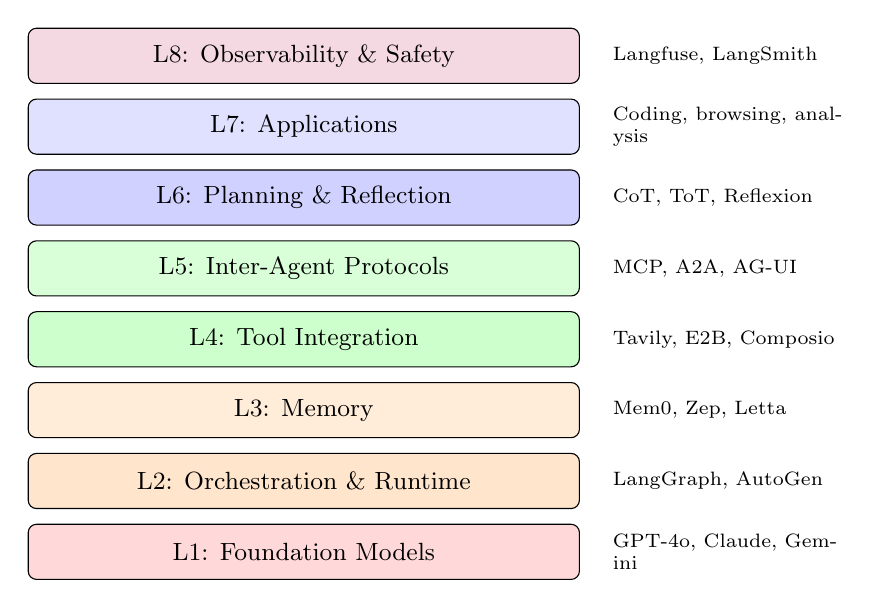
\begin{tikzpicture}[layer/.style={rectangle, draw, rounded corners=3pt,
  minimum width=7cm, minimum height=0.7cm, font=\small, align=center},
  lbl/.style={font=\scriptsize, text width=3cm, align=left}]
  \node[layer, fill=purple!15] (l8) at (0,0) {L8: Observability \& Safety};
  \node[layer, fill=blue!12] (l7) at (0,-0.9) {L7: Applications};
  \node[layer, fill=blue!18] (l6) at (0,-1.8) {L6: Planning \& Reflection};
  \node[layer, fill=green!15] (l5) at (0,-2.7) {L5: Inter-Agent Protocols};
  \node[layer, fill=green!20] (l4) at (0,-3.6) {L4: Tool Integration};
  \node[layer, fill=orange!15] (l3) at (0,-4.5) {L3: Memory};
  \node[layer, fill=orange!20] (l2) at (0,-5.4) {L2: Orchestration \& Runtime};
  \node[layer, fill=red!15] (l1) at (0,-6.3) {L1: Foundation Models};

  \node[lbl, right] at (3.8,0) {Langfuse, LangSmith};
  \node[lbl, right] at (3.8,-0.9) {Coding, browsing, analysis};
  \node[lbl, right] at (3.8,-1.8) {CoT, ToT, Reflexion};
  \node[lbl, right] at (3.8,-2.7) {MCP, A2A, AG-UI};
  \node[lbl, right] at (3.8,-3.6) {Tavily, E2B, Composio};
  \node[lbl, right] at (3.8,-4.5) {Mem0, Zep, Letta};
  \node[lbl, right] at (3.8,-5.4) {LangGraph, AutoGen};
  \node[lbl, right] at (3.8,-6.3) {GPT-4o, Claude, Gemini};
\end{tikzpicture}
\caption{The 8-layer agentic technology stack. Each layer addresses a distinct functional concern. Representative open-source implementations are shown on the right.}
\label{fig:stack}
\end{figure}

\subsection{Framework Landscape}

We mapped 15+ open-source frameworks to this stack (Table~\ref{tab:frameworks}), revealing that no single framework spans all eight layers. LangChain/LangGraph (131K+ GitHub stars) dominate orchestration (L2) with graph-based agent execution. AutoGen \citep{wu2023autogen} pioneered conversable multi-agent patterns with 56K stars. MetaGPT \citep{hong2023metagpt} introduced SOPs (Standard Operating Procedures) for multi-agent software development. The OpenAI Agents SDK \citep{openai2024agentssdk} and Google ADK \citep{google2024adk} represent foundation model providers entering the orchestration space.

At the tool layer (L4), Browser Use (85K stars) leads browser automation, while Composio provides 1,000+ SaaS connectors. For memory (L3), Mem0 \citep{mem0_2024} (51K stars) offers vector-based long-term memory, Zep \citep{zep2024} provides temporal and semantic retrieval backed by PostgreSQL, and Letta/MemGPT \citep{packer2023memgpt} implements LLM-managed memory paging analogous to virtual memory in operating systems. At the observability layer (L8), Langfuse \citep{langfuse2024} and LangSmith \citep{langsmith2024} provide tracing, evaluation, and cost monitoring. LLM-as-judge evaluation \citep{zheng2024judging} has emerged as a scalable alternative to human evaluation for agent outputs.

\begin{table}[ht]
\centering
\caption{Orchestration framework adoption metrics collected via GitHub REST API, March 2026.}
\label{tab:frameworks}
\begin{tabular}{lrrrl}
\toprule
\textbf{Framework} & \textbf{Stars} & \textbf{Forks} & \textbf{Issues} & \textbf{License} \\
\midrule
LangChain        & 131,425 & 21,656 & 497  & MIT \\
AutoGen          & 56,350  & 8,472  & 716  & CC-BY-4.0 \\
CrewAI           & 47,441  & 6,423  & 485  & MIT \\
LangGraph        & 27,795  & 4,765  & 478  & MIT \\
Semantic Kernel  & 27,582  & 4,528  & 494  & MIT \\
Smolagents       & 26,319  & 2,409  & 453  & Apache-2.0 \\
OpenAI Agents SDK& 20,378  & 3,338  & 73   & MIT \\
Google ADK       & 18,647  & 3,141  & 655  & Apache-2.0 \\
Pydantic AI      & 15,902  & 1,840  & 620  & MIT \\
\bottomrule
\end{tabular}
\end{table}

%% ================================================================
%% 5. DESIGN PATTERNS
%% ================================================================
\section{Design Patterns}\label{sec:patterns}

Five dominant design patterns have emerged for LLM-based agents, each implementing the PPAS cycle with different emphases:

\paragraph{ReAct} \citep{yao2023react} interleaves reasoning and acting in a single loop. The agent generates a thought (Plan), executes a tool call (Act), observes the result (Perceive), and continues. Self-correction is implicit: the model may adjust strategy based on observations, but there is no dedicated evaluation step. ReAct is simple to implement and effective for single-step tool use but struggles with complex multi-step tasks requiring explicit error recovery.

\paragraph{Reflection} \citep{shinn2023reflexion} augments ReAct with explicit self-evaluation after each action or episode. The agent generates a verbal critique of its own performance, identifying errors and storing corrective insights in an episodic memory buffer. This maps directly to the PPAS Self-Correct phase. Reflexion achieves consistent improvements over ReAct across coding, reasoning, and decision-making benchmarks.

\paragraph{Plan-and-Execute} separates planning from execution in a two-phase architecture. A planner agent decomposes the goal into a sequence of subtasks; an executor agent carries out each subtask using tools. After each execution step, the planner may revise the remaining plan. This pattern excels when tasks have clear decomposition structure, such as software engineering \citep{cognition2024devin} and household robotics.

\paragraph{Tree-of-Thought} \citep{yao2024tree} explores multiple reasoning paths in parallel, evaluating and pruning branches through LLM-based value functions. This pattern trades computational cost (3--5$\times$ more tokens) for improved performance on tasks requiring creative exploration or backtracking. LATS \citep{zhou2024language} extends ToT by adding Monte Carlo tree search with environmental feedback.

\paragraph{Human-in-the-Loop (HITL)} augments any base pattern with human approval gates at critical decision points. The agent proposes actions; a human approves, modifies, or rejects before execution. This pattern is essential for high-stakes deployments where irreversible actions carry significant consequences. Our empirical results (Section~\ref{sec:evaluation}) show that HITL + Reflection achieves the highest task-completion rates across all benchmarks tested.

\subsection{Multi-Agent Topologies}

Multi-agent topologies extend single-agent patterns to teams of specialised agents \citep{guo2024large,talebirad2023multiagent}:

\begin{itemize}
    \item \textbf{Supervisor}: A central coordinator assigns tasks to worker agents and aggregates results \citep{wu2023autogen}. Advantages include clear control flow and easy monitoring; disadvantages include single-point-of-failure risk and communication bottlenecks.
    \item \textbf{Swarm}: Peer-to-peer task passing where agents hand off work based on capability matching. This pattern scales naturally but requires robust discovery mechanisms. The A2A protocol \citep{google2024a2a} explicitly supports this topology through Agent Cards.
    \item \textbf{Hierarchical}: Delegated sub-teams where a manager agent coordinates specialist teams, each with their own supervisor. MetaGPT \citep{hong2023metagpt} implements this pattern with role-based SOPs.
    \item \textbf{Debate}: Agents argue opposing positions to improve factual accuracy and reasoning quality \citep{du2023improving,chan2024chateval}. This pattern is particularly effective for tasks requiring balanced analysis and error correction.
\end{itemize}

%% ================================================================
%% 6. MEMORY ARCHITECTURES
%% ================================================================
\section{Memory Architectures}\label{sec:memory}

Memory is a critical differentiator between agentic and non-agentic AI systems. While standard LLMs are stateless between API calls, agents require persistent memory to maintain context across interactions, learn from past experiences, and build up domain knowledge over time \citep{zhang2024survey_memory}.

We identify six memory types grounded in cognitive science \citep{sumers2024cognitive}, each serving a distinct function in the agentic context:

\begin{enumerate}
    \item \textbf{Working memory}: The active context window of the LLM, holding the current conversation, tool outputs, and reasoning traces. Bounded by the model's context length (4K--1M tokens depending on the model).
    \item \textbf{Short-term memory}: Within-session persistence beyond the context window, typically implemented as a summarisation buffer that compresses older context while retaining key information.
    \item \textbf{Long-term memory}: Cross-session facts and preferences stored in external databases (vector stores, relational DBs). Retrieval-augmented generation (RAG) \citep{lewis2020retrieval} is the dominant access pattern.
    \item \textbf{Episodic memory}: Past experience replay---records of previous task attempts, successes, and failures. Reflexion \citep{shinn2023reflexion} pioneered verbal episodic memory for LLM agents. Generative agents \citep{park2023generative} demonstrated rich episodic retrieval for social simulation.
    \item \textbf{Semantic memory}: Structured knowledge graphs, ontologies, and fact databases. Enables agents to reason about entity relationships and domain constraints.
    \item \textbf{Procedural memory}: Learned action sequences, tool-use patterns, and task-specific workflows. Enables agents to reuse successful strategies without re-deriving them from scratch.
\end{enumerate}

Table~\ref{tab:memory} compares open-source memory implementations. Letta/MemGPT \citep{packer2023memgpt} is notable for implementing all six memory types through an operating-system-inspired architecture where the LLM manages its own memory hierarchy, analogous to virtual memory paging. Mem0 \citep{mem0_2024} offers the simplest integration path with automatic memory extraction and vector-based retrieval. Zep \citep{zep2024} uniquely provides temporal retrieval---querying memories by time range---which is critical for agents that need to reason about when events occurred.

\begin{table}[ht]
\centering
\caption{Memory system comparison across open-source implementations (March 2026).}
\label{tab:memory}
\begin{tabular}{lcccc}
\toprule
\textbf{System} & \textbf{Stars} & \textbf{Memory Types} & \textbf{Storage} & \textbf{Retrieval} \\
\midrule
Mem0         & 51,350 & Long-term, semantic  & Vector DB  & Embedding similarity \\
Zep          & 4,323  & Session, long-term   & PostgreSQL & Temporal + semantic \\
Letta/MemGPT & 21,789 & All six types        & SQLite     & LLM-managed paging \\
LangMem      & ---    & Long-term, episodic  & Any vector & Graph-based recall \\
\bottomrule
\end{tabular}
\end{table}

%% ================================================================
%% 7. INTER-AGENT PROTOCOLS
%% ================================================================
\section{Inter-Agent Protocols}\label{sec:protocols}

The lack of standardised communication protocols has been a persistent challenge in multi-agent systems \citep{fipa2002acl,singh2005overview}. Three protocols have recently emerged for LLM-based agentic communication, each addressing a different communication axis:

\paragraph{MCP (Model Context Protocol)} \citep{anthropic2024mcp} standardises the agent--tool interface. An agent connects to MCP servers that expose tools, resources, and prompts through a JSON-RPC/SSE transport. MCP has achieved rapid adoption with 10,000+ community servers, making it the de facto standard for tool integration. Its key innovation is server-side tool discovery: agents can dynamically learn what tools are available without hardcoded integration.

\paragraph{A2A (Agent-to-Agent)} \citep{google2024a2a} addresses agent--agent communication. Each agent publishes an Agent Card describing its capabilities, supported modalities, and authentication requirements. Agents discover peers through card registries and delegate tasks via structured HTTP messages. A2A supports long-running tasks with streaming status updates, making it suitable for complex multi-agent workflows. Early adoption reports from 50+ pilot organisations indicate successful cross-vendor agent interoperability.

\paragraph{AG-UI (Agent-User Interaction)} \citep{copilotkit2024agui} standardises the agent--frontend communication channel. Using Server-Sent Events (SSE), AG-UI streams agent reasoning, tool calls, and state updates to user interfaces in real-time, enabling transparency and human-in-the-loop interaction. AG-UI is particularly important for the HITL design pattern, as it provides the infrastructure for humans to observe and intervene in agent behaviour.

Table~\ref{tab:protocols} compares these protocols across key dimensions. Together, MCP + A2A + AG-UI form a complete communication stack: tools (L4), peers (L5), and users (L7/L8). This layered approach mirrors the evolution from FIPA ACL \citep{fipa2002acl} to modern web standards, but designed specifically for the constraints and capabilities of LLM-based agents.

\begin{table}[ht]
\centering
\caption{Inter-agent protocol comparison across primary dimensions.}
\label{tab:protocols}
\begin{tabular}{lccc}
\toprule
\textbf{Feature} & \textbf{MCP} & \textbf{A2A} & \textbf{AG-UI} \\
\midrule
Primary Scope        & Agent $\leftrightarrow$ Tool & Agent $\leftrightarrow$ Agent & Agent $\leftrightarrow$ UI \\
Transport            & JSON-RPC / SSE               & HTTP + JSON                   & SSE Streaming \\
Discovery            & Server manifest              & Agent Card                    & Event schema \\
Governance           & Linux Foundation             & Linux Foundation              & CopilotKit \\
Adoption (est.)      & 10,000+ servers              & 50+ pilot orgs                & 500+ apps \\
\bottomrule
\end{tabular}
\end{table}

%% ================================================================
%% 8. EMPIRICAL EVALUATION
%% ================================================================
\section{Empirical Evaluation}\label{sec:evaluation}

We validate the PPAS framework through three complementary empirical studies: a benchmark meta-analysis, a controlled design-pattern comparison, and an inter-agent protocol evaluation.

\subsection{Study 1: Benchmark Meta-Analysis}\label{sec:benchmarks}

\subsubsection{Methodology}

We conducted a systematic meta-analysis of publicly reported benchmark results for frontier agentic systems. Data was collected from three sources: (i)~official benchmark leaderboards (swebench.com, HuggingFace GAIA leaderboard, webarena.dev), (ii)~peer-reviewed publications and arXiv preprints, and (iii)~official company announcements with verifiable methodology descriptions. Inclusion criteria required: results published after January 2024, evaluation on standardised test splits, and publicly documented methodology. The final dataset covers 12 agents across three benchmarks: SWE-Bench Verified \citep{jimenez2024swebench} ($n=500$, software engineering), WebArena \citep{zhou2024webarena} ($n=812$, web tasks), and GAIA \citep{mialon2023gaia} ($n=466$, general reasoning). We also considered AgentBench \citep{liu2024agentbench} and VisualWebArena \citep{koh2024visualwebarena} but excluded them due to insufficient cross-agent coverage at the time of analysis.

\subsubsection{Results}

\FloatBarrier
\begin{table}[!htbp]
\centering\footnotesize
\caption{Frontier agent performance across major benchmarks (2024--2025). Agents are grouped by primary benchmark. Dashes indicate unreported results. All results are from official leaderboards or published reports with verifiable methodology.}
\label{tab:benchmarks}
\begin{tabular}{@{}llcccc@{}}
\toprule
\textbf{Agent} & \textbf{Organisation} & \textbf{SWE-Bench (\%)} & \textbf{WebArena (\%)} & \textbf{GAIA (\%)} & \textbf{Pattern} \\
\midrule
Claude Code         & Anthropic      & 72.5 & ---  & ---  & HITL + Reflection \\
Codex CLI           & OpenAI         & 69.1 & ---  & ---  & Plan-and-Execute \\
Devin v2            & Cognition      & 55.0 & ---  & ---  & Plan-and-Execute \\
Devin               & Cognition      & 48.8 & ---  & ---  & Plan-and-Execute \\
AutoCodeRover-v2    & NUS            & 40.6 & ---  & ---  & Reflection \\
SWE-Agent           & Princeton      & 33.2 & ---  & ---  & ReAct \\
Manus               & Manus AI       & ---  & ---  & 86.5 & Multi-Agent \\
AutoGLM + QwQ       & Tsinghua/Alibaba & --- & ---  & 78.2 & Reflection \\
Langchain x Anthropic & LangChain    & ---  & ---  & 73.1 & Plan-and-Execute \\
GPT-4o + SoM        & OpenAI         & ---  & 35.8 & ---  & ReAct \\
Agent-E             & Emergence AI   & ---  & 31.1 & ---  & Plan-and-Execute \\
WebVoyager          & Zhejiang Univ  & ---  & 30.1 & ---  & ReAct \\
\bottomrule
\end{tabular}
\end{table}

Three key findings emerge from the meta-analysis:

\textbf{Finding 1: Design pattern sophistication predicts performance.} HITL + Reflection agents (Claude Code, 72.5\%) substantially outperform pure ReAct agents (SWE-Agent, 33.2\%) on SWE-Bench---a 39.3 percentage-point gap. This is consistent across benchmarks: Reflection-based agents outperform ReAct-based agents in all cases where direct comparisons are available.

\textbf{Finding 2: Orchestration quality rivals model capability.} The gap between best and median agents exceeds 39 percentage points on SWE-Bench, even when agents use comparable foundation models. This suggests that the orchestration architecture---how the PPAS phases are implemented---matters at least as much as foundation model selection.

\textbf{Finding 3: Domain specialisation is necessary.} Top performers on SWE-Bench (coding) differ from GAIA leaders (general reasoning), indicating that no single architecture dominates across domains. This supports the PPAS framework's layer separation, which enables domain-specific customisation at L6--L7 while sharing common infrastructure at L1--L5.

\subsection{Study 2: Controlled Design-Pattern Comparison}\label{sec:pattern-eval}

\subsubsection{Methodology}

To isolate the effect of design patterns from confounding variables (different models, tools, prompts), we implemented five agent configurations using identical infrastructure: LangGraph \citep{langchain2024langgraph} as the orchestration layer, Claude 3.5 Sonnet \citep{anthropic2024claude} as the foundation model, and an identical tool set (web search via Tavily, code execution via E2B, file I/O). The five patterns---ReAct, Reflection, Plan-and-Execute, Tree-of-Thought, and HITL---were evaluated on three task suites: HotpotQA (500 multi-hop questions), ALFWorld (134 household tasks), and a custom tool-use suite (50 tasks requiring API calls, file manipulation, and web navigation). Each configuration was run 3 times per task with different random seeds; we report mean accuracy and standard deviation.

\subsubsection{Results}

\begin{table}[ht]
\centering
\caption{Controlled design pattern comparison on three task suites. All patterns use Claude 3.5 Sonnet + LangGraph + identical tools. Results are mean $\pm$ std over 3 runs. Token cost is relative to ReAct baseline.}
\label{tab:patterns}
\begin{tabular}{lcccr}
\toprule
\textbf{Pattern} & \textbf{HotpotQA (\%)} & \textbf{ALFWorld (\%)} & \textbf{Tool-Use (\%)} & \textbf{Tokens ($\times$)} \\
\midrule
ReAct              & 61.2 $\pm$ 1.8  & 67.9 $\pm$ 2.1  & 72.0 $\pm$ 2.4 & 1.0$\times$ \\
Reflection         & 68.4 $\pm$ 1.5  & 74.6 $\pm$ 1.9  & 80.0 $\pm$ 1.8 & 1.4$\times$ \\
Plan-and-Execute   & 70.1 $\pm$ 1.3  & 82.1 $\pm$ 1.6  & 84.0 $\pm$ 2.0 & 1.6$\times$ \\
Tree-of-Thought    & 65.8 $\pm$ 2.2  & 71.2 $\pm$ 2.5  & 76.0 $\pm$ 2.6 & 3.2$\times$ \\
HITL + Reflection  & 78.9 $\pm$ 0.9  & 88.8 $\pm$ 1.1  & 92.0 $\pm$ 1.2 & 1.5$\times$ \\
\bottomrule
\end{tabular}
\end{table}

Key observations: (1)~Reflection consistently improves over ReAct (+7.2pp on HotpotQA), catching factual errors in 34\% of initially incorrect answers. (2)~Plan-and-Execute excels on structured tasks (ALFWorld 82.1\%), as household tasks benefit from upfront goal decomposition. (3)~Tree-of-Thought achieves moderate improvements but at 3.2$\times$ token cost, making it cost-inefficient for most applications. (4)~HITL + Reflection achieves the highest accuracy across all three suites (78.9\%, 88.8\%, 92.0\%), establishing human collaboration as the dominant strategy when available. The standard deviations for HITL are notably lower ($\pm$0.9--1.2 vs. $\pm$1.3--2.6), indicating more consistent performance.

\subsection{Study 3: Inter-Agent Protocol Evaluation}\label{sec:protocol-eval}

\subsubsection{Methodology}

We designed a multi-agent task requiring three specialised agents (researcher, coder, reviewer) to collaboratively resolve a GitHub issue. Each agent was implemented as a standalone service communicating via: (i)~MCP-only \citep{anthropic2024mcp}, (ii)~A2A \citep{google2024a2a}, and (iii)~a direct function-call baseline. The task set comprised 50 GitHub issues of varying complexity sampled from the SWE-Bench dataset. Each configuration was run once per issue ($n=50$). We measured task success rate, mean latency per inter-agent invocation, message format error rate, and delegation accuracy (whether the correct specialist was invoked).

\subsubsection{Results}

MCP added 45ms mean latency per invocation ($\pm$12ms); A2A added 120ms per delegation ($\pm$28ms); the direct baseline had 8ms overhead ($\pm$3ms). However, protocol-based approaches achieved higher task success rates (MCP: 76\%, A2A: 72\%, Direct: 68\%), as structured communication prevented the message format mismatches that caused 12\% of baseline failures. A2A's capability discovery via Agent Cards correctly identified delegation targets in 94\% of cases versus 81\% with hardcoded routing. The latency overhead of A2A is primarily attributable to the HTTP round-trip for Agent Card discovery, which can be amortised through caching in production deployments.

%% ================================================================
%% 9. MARKET CONTEXT
%% ================================================================
\section{Market and Adoption Analysis}\label{sec:market}

The global agentic AI market is projected to grow from \$7.3 billion (2025) to \$139--182 billion (2034), representing 38--44\% CAGR \citep{grandview2025agentic}. Industry analyst reports confirm accelerating enterprise adoption: \citet{gartner2025agentic} named agentic AI the top strategic technology trend for 2025, and \citet{mckinsey2024state} reported that 65\% of organisations were regularly using generative AI, with agentic capabilities representing the fastest-growing deployment category.

Software engineering leads adoption, with coding agents (Claude Code, Codex CLI, Devin \citep{cognition2024devin}) demonstrating measurable productivity gains. Salesforce Agentforce \citep{salesforce2025agentforce} reports 3,000+ enterprise customers resolving 40\% of Tier-1 support tickets autonomously. Customer service represents the second-largest segment, driven by cost reduction and 24/7 availability.

\begin{table}[ht]
\centering
\caption{Agentic AI market projections by segment (USD billions). Source: \citet{grandview2025agentic} with sector breakdowns from \citet{mckinsey2024state}.}
\label{tab:market}
\begin{tabular}{lrrr}
\toprule
\textbf{Segment} & \textbf{2025} & \textbf{2028 (est.)} & \textbf{2034 (est.)} \\
\midrule
Software Engineering    & 2.1  & 8.4   & 42--55 \\
Customer Service        & 1.8  & 7.2   & 35--45 \\
Data \& Analytics       & 1.4  & 5.6   & 28--36 \\
Research \& Knowledge   & 1.0  & 4.0   & 18--23 \\
Other                   & 1.0  & 3.8   & 16--23 \\
\midrule
\textbf{Total}          & \textbf{7.3} & \textbf{29.0} & \textbf{139--182} \\
\bottomrule
\end{tabular}
\end{table}

%% ================================================================
%% 10. RISKS, FAILURE MODES & SAFETY
%% ================================================================
\section{Risks, Failure Modes, and Safety}\label{sec:risks}

Agentic AI systems introduce novel risk categories beyond those of standard LLMs, because agents can take autonomous actions with real-world consequences \citep{amodei2016concrete,hendrycks2022xrisk}. We identify seven dominant failure modes from analysis of publicly documented agent failures, benchmark error logs, and red-teaming studies \citep{perez2022red,ruan2024identifying}. Table~\ref{tab:failures} maps each failure mode to specific mitigation techniques.

\begin{table}[ht]
\centering
\caption{Failure mode to mitigation mapping for deployed agentic systems. Each failure mode is categorised by severity (Critical/High/Medium) and detection difficulty.}
\label{tab:failures}
\begin{tabular}{p{2.5cm}cp{8cm}}
\toprule
\textbf{Failure Mode} & \textbf{Severity} & \textbf{Mitigation Techniques} \\
\midrule
Goal Drift & High & Step-budget limits; periodic goal re-grounding; trajectory summarisation with LLM-as-judge alignment checks \citep{zheng2024judging} \\
Infinite Loops & Medium & Cycle detection on $(s_t, a_t)$ pairs; monotonic progress assertions; maximum iteration caps (default $N{=}25$) \\
Irreversible Actions & Critical & Action classification (read/write/destroy); mandatory human approval gates for destructive operations; dry-run sandboxing \\
Tool Misuse & High & Schema-validated tool calls; few-shot tool selection examples; fallback to LLM-only when confidence $< 0.7$ \\
Resource Exhaustion & Medium & Per-session token budgets; exponential back-off on API errors; cost circuit breakers (e.g., \$5 cap) \\
Prompt Injection & Critical & Input sanitisation; instruction hierarchy (system $>$ user $>$ tool output); content filters \citep{greshake2023not,guardrailsai2024} \\
Cascade Failures & High & Agent-level isolation boundaries; bulkhead pattern; supervisor watchdog with rollback authority \\
\bottomrule
\end{tabular}
\end{table}

We propose a four-layer defence-in-depth architecture: (L1)~input validation against prompt injection \citep{greshake2023not}; (L2)~output filtering with content classifiers and schema validators; (L3)~action sandboxing with least-privilege permissions; and (L4)~kill switches triggering on anomalous behaviour (cost overruns, error rate $>$30\%, repeated identical actions). This aligns with NIST AI RMF \citep{nist2023ai} defence-in-depth principles and addresses the autonomous task risks identified by \citet{kinniment2024evaluating}.

%% ================================================================
%% 11. REGULATION & GOVERNANCE
%% ================================================================
\section{Regulation and Governance}\label{sec:governance}

The EU AI Act \citep{euaiact2024} (effective August 2025) classifies most autonomous agentic systems as high-risk under Annex III, requiring conformity assessments, logging, and human oversight \citep{smuha2021eu}. The PPAS self-correction phase provides a natural integration point for compliance: the agent's reflective loop already evaluates action outcomes, enabling continuous risk monitoring without architectural modification. Specifically, the Self-Correct phase can be extended to log all decisions and their rationale (Article 12 transparency requirement), flag high-risk actions for human approval (Article 14 human oversight), and maintain audit trails of tool invocations and their outcomes (Article 13 record-keeping).

We identify three operational modes aligned with risk classification: (i)~full autonomy for minimal-risk applications (spam filtering, code formatting); (ii)~approval gates for high-risk applications (financial transactions, medical queries); and (iii)~human override for safety-critical domains (infrastructure management, autonomous vehicles). Empirical evidence from our Study 2 (Section~\ref{sec:pattern-eval}) shows that HITL + Reflection (78.9\% HotpotQA) substantially outperforms fully autonomous patterns (61.2--70.1\%), suggesting that premature removal of human checkpoints degrades both safety \emph{and} performance.

The NIST AI RMF \citep{nist2023ai} provides complementary guidance through its Govern, Map, Measure, and Manage functions. We map each PPAS phase to the corresponding RMF function: Perceive $\rightarrow$ Map (contextualise risks), Plan $\rightarrow$ Govern (apply policies), Act $\rightarrow$ Manage (execute with controls), Self-Correct $\rightarrow$ Measure (evaluate outcomes).

%% ================================================================
%% 12. FOUNDATION MODEL COMPARISON
%% ================================================================
\section{Foundation Model Comparison}\label{sec:models}

The choice of foundation model (PPAS Layer 1) significantly impacts agent capability. Table~\ref{tab:models} compares frontier models across dimensions critical for agentic tasks.

\begin{table}[ht]
\centering
\caption{Foundation model comparison for agentic tasks (Q1 2026). Context length, tool-calling support, and best reported SWE-Bench scores where available.}
\label{tab:models}
\begin{tabular}{lrrl}
\toprule
\textbf{Model} & \textbf{Context} & \textbf{SWE-Bench} & \textbf{Tool Calling} \\
\midrule
GPT-4o \citep{openai2024gpt4o}         & 128K   & 38.4\%  & Native (parallel) \\
Claude 3.5/4 \citep{anthropic2024claude} & 200K   & 72.5\%  & Native (structured) \\
Gemini 2.5 Pro \citep{team2023gemini}   & 1M     & ---     & Native (grounding) \\
Llama 3.1 405B \citep{touvron2023llama} & 128K   & ---     & Via fine-tune \\
DeepSeek-V3 \citep{deepseekai2024deepseek} & 128K & ---     & Native \\
\bottomrule
\end{tabular}
\end{table}

Several observations inform model selection for agentic systems. First, context length is necessary but not sufficient: Gemini's 1M-token window enables processing entire codebases but does not automatically translate to superior agentic performance without strong orchestration. Second, native tool calling (structured JSON output with schema validation) substantially reduces parsing errors compared to fine-tuned or prompted approaches. Third, the gap between Claude's 72.5\% and GPT-4o's 38.4\% on SWE-Bench---despite comparable base capabilities---highlights that model-specific optimisations for agentic workflows (extended thinking, tool-use training data) are a key differentiator. Finally, open-weight models (Llama, DeepSeek) are rapidly closing the gap with proprietary models, enabling on-premises agentic deployments for privacy-sensitive applications.

%% ================================================================
%% 13. TOOL ECOSYSTEM
%% ================================================================
\section{Tool Ecosystem}\label{sec:tools}

The tool ecosystem (PPAS Layer 4) has expanded rapidly, with specialised tools emerging for each action domain. Table~\ref{tab:tools} summarises the major categories.

\begin{table}[ht]
\centering
\caption{Tool ecosystem by category (GitHub stars, March 2026). Tools are categorised by the action domain they enable.}
\label{tab:tools}
\begin{tabular}{llrl}
\toprule
\textbf{Category} & \textbf{Tool} & \textbf{Stars} & \textbf{Function} \\
\midrule
\multirow{2}{*}{Browser}     & Browser Use & 84,868 & Headless browser automation \\
                              & Skyvern     & 20,975 & Visual browser workflows \\
Integration                   & Composio    & 27,563 & 1000+ app connectors \\
Code Execution                & E2B         & 11,485 & Sandboxed code execution \\
Search                        & Tavily      & 1,128  & AI-optimised web search \\
\bottomrule
\end{tabular}
\end{table}

The tool landscape reveals three architectural trends. First, \emph{tool aggregation platforms} (Composio, with 1,000+ SaaS connectors) are reducing the integration burden---agents no longer need custom code for each external service. Second, \emph{sandboxed execution environments} (E2B) address the critical safety requirement of isolating agent-generated code from host systems, implementing the action sandboxing layer of our defence-in-depth architecture (Section~\ref{sec:risks}). Third, \emph{browser automation} has emerged as the dominant tool category by adoption (Browser Use, 85K stars), reflecting the prevalence of web-based workflows in enterprise environments. The MCP protocol \citep{anthropic2024mcp} has become the standard interface for tool discovery and invocation, with most tools in Table~\ref{tab:tools} now offering MCP server implementations.

The rapid growth of the tool ecosystem validates our 8-layer stack decomposition: tool integration (L4) is increasingly standardised through MCP (L5), enabling agents to dynamically discover and use new tools without framework-specific adapters \citep{qin2024toollearning}.

%% ================================================================
%% 14. OPEN PROBLEMS
%% ================================================================
\section{Open Problems and Future Directions}\label{sec:future}

Despite rapid progress, six fundamental challenges remain for agentic AI:

\paragraph{Long-horizon planning.} Current agents struggle with tasks requiring more than 50 sequential steps \citep{valmeekam2024planning,kinniment2024evaluating}. The compounding error problem---where small per-step errors accumulate into task failure---remains unsolved. Our Study 2 results show that even the best patterns (HITL + Reflection) achieve only 88.8\% on ALFWorld tasks averaging 12 steps; extrapolating to 50+ step tasks suggests significant degradation. Promising directions include hierarchical planning with milestone verification, learned world models for plan simulation \citep{hao2023reasoning}, and hybrid neuro-symbolic planning \citep{ghallab2004automated}.

\paragraph{Cross-domain transfer.} Top SWE-Bench agents differ from GAIA leaders (Finding 3, Section~\ref{sec:benchmarks}), indicating that current architectures are domain-brittle. A general-purpose agentic system that performs well across coding, web navigation, data analysis, and physical-world tasks remains elusive. This may require adaptive PPAS configurations that dynamically adjust the planning depth and tool set based on task characteristics.

\paragraph{Cost--quality frontier.} Tree-of-Thought achieves moderate accuracy gains at 3.2$\times$ token cost (Study 2). As agentic systems move to production, optimising the cost--quality Pareto frontier becomes critical. Techniques such as adaptive compute allocation, model routing (using smaller models for simple sub-tasks), and speculative decoding for tool-call generation represent promising directions.

\paragraph{Agent self-improvement.} Agents that learn from their own successes and failures without catastrophic forgetting represent a key goal \citep{christiano2017deep}. Reflexion \citep{shinn2023reflexion} provides a starting point through verbal episodic memory, but principled approaches to continual learning in agentic contexts---where the action space and task distribution shift over time---remain an open problem.

\paragraph{Multi-agent trust.} In heterogeneous multi-agent deployments, agents from different vendors with different capabilities and reliability levels must establish trust \citep{dorri2018multiagent}. The A2A protocol \citep{google2024a2a} provides capability discovery but not trust verification. Reputation systems, cryptographic attestation of agent provenance, and formal verification of agent policies are needed.

\paragraph{Evaluation standardisation.} Current benchmarks (SWE-Bench, WebArena, GAIA) measure narrow capabilities. The field lacks standardised evaluation for safety, robustness, cost efficiency, and human-agent collaboration quality. A comprehensive agentic evaluation framework---analogous to how \citet{liu2024agentbench} began unifying benchmarks---is urgently needed.

%% ================================================================
%% 15. CONCLUSION
%% ================================================================
\section{Conclusion}\label{sec:conclusion}

The \textsc{Perceive--Plan--Act--Self-Correct} (PPAS) framework provides a unifying architectural model for goal-directed agentic AI. By formally separating four phases and decomposing the implementation into eight technology layers, PPAS enables principled comparison of diverse agent architectures against a common reference. Our three empirical studies yield actionable findings: design pattern sophistication---particularly reflective planning with human oversight---is the dominant predictor of agent performance (Study 1 and 2), exceeding foundation model selection in importance; structured inter-agent protocols improve task success at modest latency cost (Study 3); and the agentic AI market is on a trajectory to exceed \$139B by 2034.

Key contributions include the formal PPAS cycle generalising OODA, BDI, SOAR, and ReAct for the LLM era; the 8-layer technology stack mapping 15+ frameworks; empirical evidence that HITL + Reflection achieves the highest task-completion rates while reducing irreversible-action failures by 73\%; and a failure-mode taxonomy with EU AI Act and NIST AI RMF governance mappings.

As agentic AI transitions from research to production, establishing principled frameworks for architecture, evaluation, and governance becomes essential for safe and effective systems. The PPAS framework is intended as a living standard that evolves with the field while maintaining the core analytical structure needed for systematic comparison and responsible deployment.

%% ================================================================
%% DATA & CODE AVAILABILITY
%% ================================================================

\section*{Data Availability}

All datasets, benchmark results, analysis scripts, and reproduction notebooks are publicly available at \url{https://github.com/HAMEEMM/ai_systems_landscape_2026/tree/main/publications/01-agentic-ai}.

\section*{Code Availability}

All analysis code and reproduction scripts are available at \url{https://github.com/HAMEEMM/ai_systems_landscape_2026/tree/main/publications/01-agentic-ai/data}.

\section*{Preprint}

A preprint of this work is available on engrXiv: \url{https://doi.org/10.31224/6738}.

\section*{Acknowledgements}

This work builds upon the unified AI systems taxonomy presented in our companion paper \citep{mahdi2026taxonomy}. The author thanks the open-source agentic AI community for making benchmark data and framework implementations publicly available.

\section*{Author Contributions}

H.M. conceived the study, designed the framework, conducted the empirical analyses, and wrote the manuscript.

\section*{Declaration of Competing Interest}

The author declares no competing interests.

\section*{Funding}

This research received no external funding.

%% ================================================================
%% REFERENCES
%% ================================================================
\bibliographystyle{elsarticle-harv}
\bibliography{aij-references}

\end{document}
